\documentclass{templateApunte}
\usepackage{tcolorbox}
% \usepackage{geometry}
\usepackage{pdflscape}

\definecolor{Violeta}{RGB}{124,0,254}
\definecolor{Verde2}{RGB}{130,254,0} % Complementario
\definecolor{Naranja2}{RGB}{254,124,0} % Triadico
\definecolor{Verde3}{RGB}{0,254,124} % Triadico

\definecolor{Amarillo}{RGB}{249,228,0}
\definecolor{Azul2}{RGB}{0,21,249} % Complementario
\definecolor{Celeste2}{RGB}{0,249,228} % Triadico
\definecolor{Rosa}{RGB}{228,0,249} % Triadico

\definecolor{Naranja}{RGB}{255,175,0}
\definecolor{Azul3}{RGB}{0,80,255} % Complementario
\definecolor{Cian}{RGB}{0,255,175} % Triadico
\definecolor{Violeta2}{RGB}{175,0,255} % Triadico

\definecolor{Rojo}{RGB}{245,0,79}
\definecolor{Verde4}{RGB}{0,245,166} % Complementario
\definecolor{Verde}{RGB}{79,245,0} % Triadico
\definecolor{Azul}{RGB}{0,79,245} % Triadico

\definecolor{Celeste}{RGB}{0,191,255}
\definecolor{Salmon}{RGB}{255,0,157}

\newcommand{\newparagraph}{\par\vspace{\baselineskip}\noindent}
\newcommand{\hlcolor}[2]{{\sethlcolor{#1}\hl{#2}}}

\tcbuselibrary{skins}
\usetikzlibrary{shadings}
\newcounter{counter_comentario}
\newcounter{counter_observacion}
\tcbset{
  base/.style={
    empty,
    frame engine=path,
    colframe=white,
    sharp corners,
    %title={Comentario \thetcbcounter},
    attach boxed title to top left={yshift*=-\tcboxedtitleheight},
    boxed title style={size=minimal, top=4pt, left=4pt},
    coltitle=black,
    fonttitle=\large\it,
  }
}
\newtcolorbox{cP}[5]{%
  base,
  title={#3 \csname the#2\endcsname}, % Título personalizado #2 = nombre contador ; #3 = Título
  drop fuzzy shadow, % Sombra del cuadro de texto
  coltitle=#1,
  borderline west={3pt}{-3pt}{#4}, % Borde Izquierdo #4 = color del borde
  attach boxed title to top left={xshift=-3mm, yshift*=-\tcboxedtitleheight/2},
  boxed title style={right=3pt, bottom=3pt, overlay={
    \draw[draw=#5, fill=#5, line join=round]
      (frame.south west) -- (frame.north west) -- (frame.north east) --
      (frame.south east) -- ++(-2pt, 0) -- ++(-2pt, -4pt) --
      ++(-2pt, 4pt) -- cycle; % #5 = color del fondo
  }}, % Cuadro de titulo
  overlay unbroken={
    \scoped \shade[left color=#5!30!black, right color=#5]
    ([yshift=-0.2pt]title.south west) -- ([xshift=-3pt, yshift=-0.2pt]title.south-|frame.west) -- ++(0, -4pt) -- cycle;
  }, % Sombra de titulo #5 = color del titulo
  before upper={\stepcounter{#2}}
}
\newtcolorbox{cPB}[2]{%
  base,
  coltitle=#1,
  % drop fuzzy shadow, % Sombra del cuadro de texto
  borderline west={3pt}{-3pt}{#2}, % Borde Izquierdo #4 = color del borde
}
\begin{document}
% Seteo de contadores a 1
\setcounter{counter_comentario}{1}
\setcounter{counter_observacion}{1}

\imagenlogoU{img/LogoElNube.png}
\linklogoU{https://github.com/MarceloPazPezo}
\linkQRDoc{https://github.com/MarceloPazPezo/MyRepo/blob/main/Icinf/Semestre-8/Ingenieria-de-Software/BPMN/Ejercicios_BPMN.pdf}
\titulo{Ejercicios BPMN}
\asignatura{Ingeniería de Software}
\autor{
Marcelo Paz
}
\vDoc{1.0.1}
\tipoDoc{Resolución}

% Metadatos del PDF
\title{[\asignatura]-\titulo}
\author{
    \autor
}
\portada
\margenes % Crear márgenes

\section{Caso 1: LeeRapidito}
\subsection{Enunciado:}
La empresa LeeRapidito es una empresa internacional que ofrece un curso de lectura veloz a niños 
desde los 8 años hasta adultos de 60 años.
\begin{itemize}
  \item El curso está dividido en 20 módulos, como mínimo el curso termina en 20 semanas, una para cada módulo.
  \item Al terminar el curso el alumno debe leer como  mínimo 2000 palabras por minuto (PxM) con un 100\% de comprensión lectora (CL).
  \item Para pasar un módulo el alumno debe realizar una serie de ejercicios tres veces al día y debe cumplir con el estándar mínimo de módulo, en cuanto a la cantidad de PxM y \% de CL.
  \item Cuando un cliente compra el servicio, el agente le entrega copia del comprobante de pago y el número de matrícula.
  \item El alumno, con su número de matrícula pide hora para la clase.
  \item En esta clase el profesor explica la técnica de lectura, aplica una evaluación y explica detalladamente los ejercicios que el alumno deberá desarrollar como practica para pasar al módulo 2.
  \item Los resultados de su evaluación (PxM y \% de CL) son registrados por el profesor en una hoja de asistencia y en el formulario de práctica.
  \item En este formulario el alumno anotará los resultados de sus ejercicios diarios.
  \item En el formulario el profesor debe anotar también el tiempo de duración de cada ejercicio y el mínimo o máximo que el alumno debe alcanzar en cada uno.
  \item Para las siguientes clases el alumno debe pedir, con su número de matrícula, una hora, nunca antes de 5 días ya que debe cumplir con las prácticas de los ejercicios requeridos por cada módulo.
  \item En cada clase el profesor comienza revisando que el alumno cumplió con los ejercicios, para eso revisa el formulario de práctica, el alumno debe llevar, por lo menos, 15 practicas registradas para cada uno de los ejercicios indicados para el módulo.
  \item Luego el profesor realiza una evaluación donde se verifica si el alumno puede continuar al siguiente módulo.
  \item En aquellos casos en los que el alumno no tiene el formulario de practica completo o correcto el profesor puede reprobarlo o pasarlo de módulo, esto depende del rendimiento del alumno en la evaluación y de la importancia de los ejercicios que el alumno no realizó o realizó mal.
  \item Si el profesor decide pasarlo de módulo deberá agregarle ejercicios adicionales para que alumno practique.
  \item Al terminar el módulo 20 el profesor aplica la última evaluación, si el alumno cumple con las exigencias del curso pasará a ser un egresado, el profesor lo registra en el libro de egresados y le pedirá una carta donde indique los logros y beneficios que ha alcanzado y espera alcanzar en el futuro gracias a la técnica de lectura aprendida.
  \item Si el alumno reprueba la evaluación final deberá repetir el último curso, tal y como antes.
  \item Los alumnos que no logren terminar el curso en 10 meses deberán pedir, a través de una carta a la directora de la sede la autorización para continuar.
  \item La directora notifica su respuesta al alumno, de ser aprobada el alumno puede retomar sus cursos durante el mes, de no ser aprobada el alumno deja de ser un alumno vigente.
  \item Los alumnos que logran ser lectores profesionales, sean niños o adultos, tienen grandes beneficios en su vida académica y profesional, sin mencionar los beneficios que se ganan por el solo hecho de fomentar la lectura en general. 
\end{itemize}
Actualmente, la empresa cuenta solo con el libro de asistencia para controlar el progreso de cada alumno, pero la cantidad de información manejada hace casi imposible detectar algunos hechos como la inasistencia prolongada, el incumplimiento del número de prácticas, repeticiones frecuentes de cursos, etc.
Para la empresa es importante que todos los alumnos cumplan con el curso en el mínimo tiempo, aunque sin sacrificar los objetivos finales de éste.
Hoy día es difícil atender a padres que llegan a consultar por el rendimiento o asistencia de un alumno, emitir boletines con los promedios diarios de PxM y \% de CL por sede, et.
Por ejemplo, si el alumno pierde su formulario queda automáticamente reprobado del módulo ya que no existen registros de sus prácticas. 
\newparagraph
La empresa XSTO ha ganado gran prestigio en el ámbito Financiero y Forestal con el desarrollo de software de control automático de la producción de paneles y maderas prensadas. Cuenta con un equipo de 3 programadores, con vasta experiencia en PHP, los cuales llevan 2 años trabajando en la empresa.Usted es el ingeniero contratado para liderar el proyecto dada su experiencia en desarrollado web y nuevas tecnologías como MERN. 

\newpage
\begin{landscape}
  \subsection{BPMN: }
  \begin{figure}[H]
    \centering
    \includegraphics[width=24cm]{img/LeeRapidito.png}
  \end{figure}
\end{landscape}

\section{Caso 2: Pillan}
\subsection{Enunciado:}
Pillan se preocupa de entregar productos con carácter propio, combinando las maderas más nobles, fierro forjado, cerámicos, entre otros materiales. Debido a que los muebles son fabricados en bajas cantidades por cada diseño, para realizar las ventas en los locales se utiliza un catálogo con los productos que se encuentran en la Fábrica.
\begin{itemize}
  \item Si el cliente elige un producto del catálogo, se realiza la venta y se emite una orden de despacho al encargado de bodega de la fábrica, quien debe embalar el producto y enviar el producto al cliente a través una empresa de transporte.
  \item Cuando el transportista notifica la entrega al encargado de despacho se cierra ese pedido.
  \item Si el cliente desea un nuevo diseño, el vendedor registra el pedido del cliente, las medidas, las características, los materiales y el boceto del producto solicitado y lo envía a la fábrica.
  \item El encargado de fabricación recibe el pedido y analiza la disponibilidad de materiales, prepara un diseño formal, estima los costos ...
\end{itemize}

\subsection{BPMN:}
\begin{figure}[H]
  \centering
  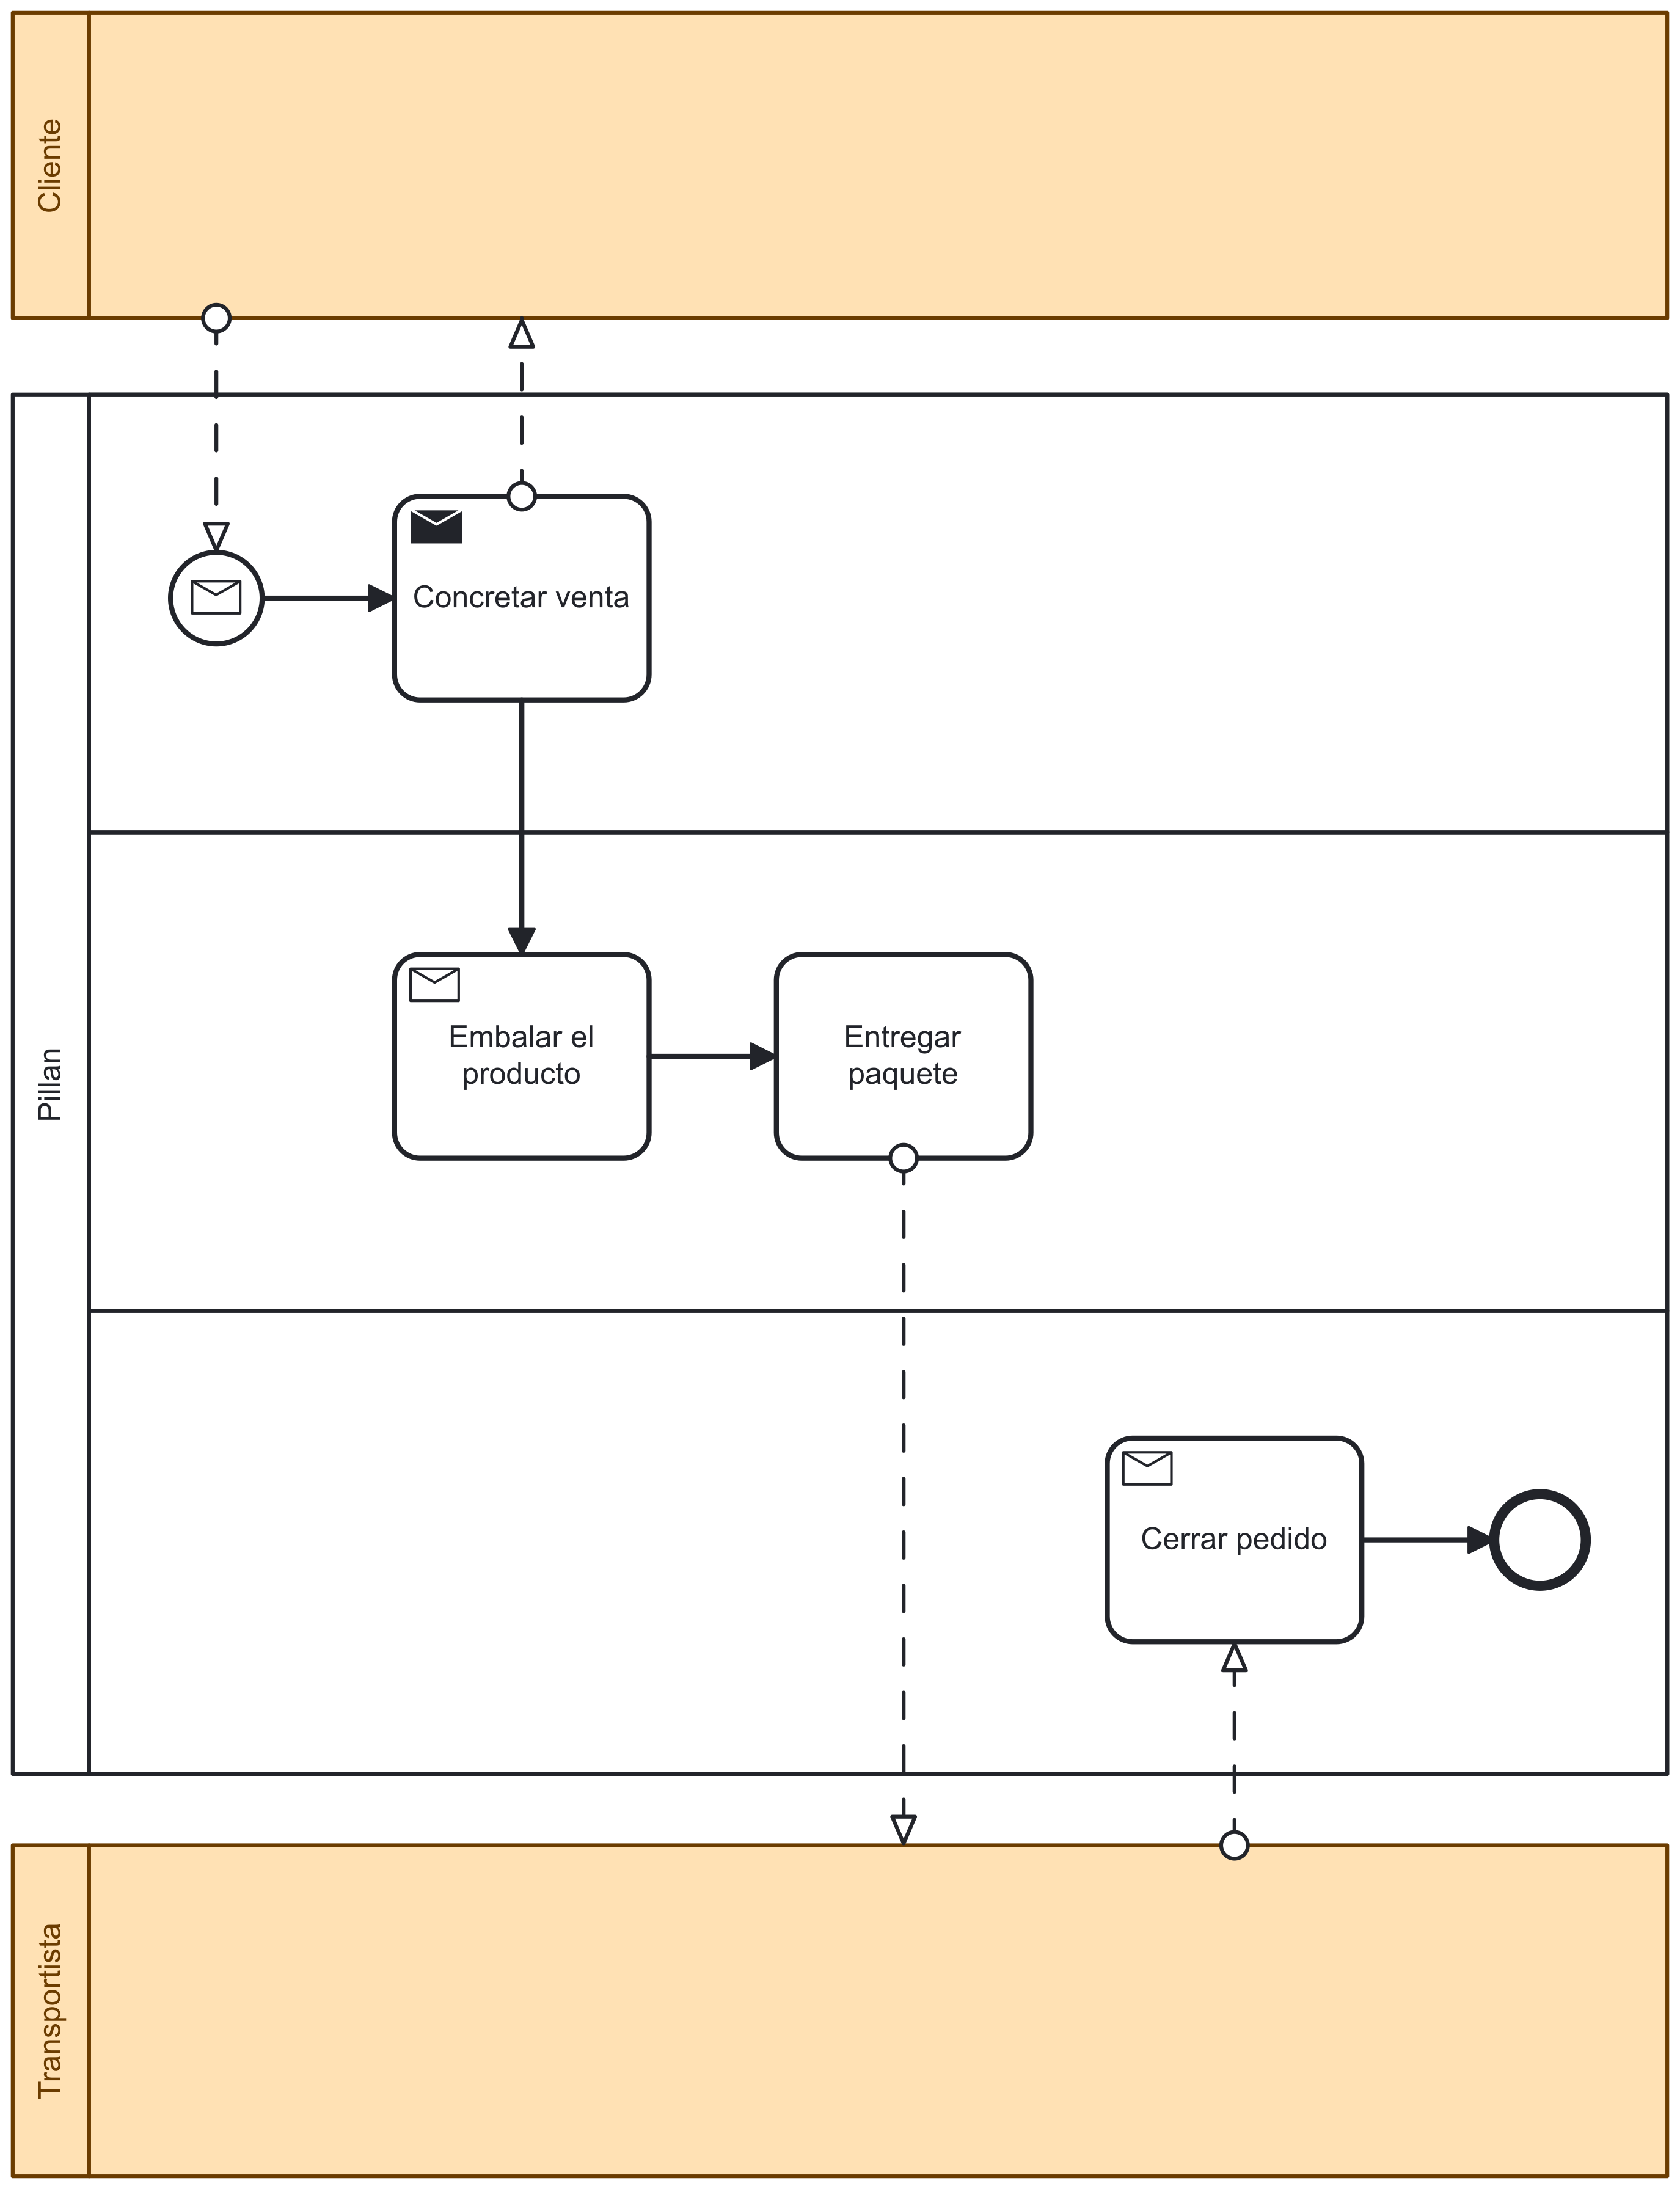
\includegraphics[width=0.55\textwidth]{img/Pillan.png}
\end{figure}
\end{document}